% !TEX root = ../../statikz/statikz.tex

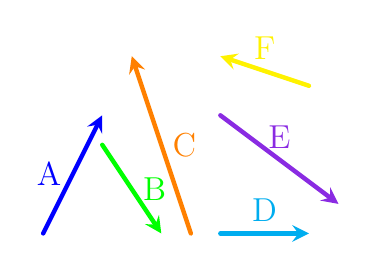
\begin{tikzpicture}[scale =0.75, style={line cap = round}]
  % \filldraw [white, draw=saitMaroon, thick, drop shadow={opacity=0.25}] (0.5, 0.5) rectangle (6.5,4.5);
  \draw[ultra thick, blue, ->, >=stealth] (1, 1) -- node[left] {\large ${\bm{\mathrm{ A }}}$} ++(1, 2);
  \draw[ultra thick, green, ->, >=stealth] (2, 2.5) -- node[right]{\large ${\bm{\mathrm{ B }}}$} ++ (1, -1.5);
  \draw[ultra thick, orange, ->, >=stealth] (3.5, 1) -- node[right]{\large ${\bm{\mathrm{ C }}}$} ++ (-1, 3);
  \draw[ultra thick, cyan, ->, >=stealth] (4, 1) -- node[above]{\large ${\bm{\mathrm{ D }}}$} ++ (1.5, 0);
  \draw[ultra thick, BlueViolet, ->, >=stealth] (4, 3) -- node[above]{\large ${\bm{\mathrm{ E }}}$} ++ (2, -1.5);
  \draw[ultra thick, yellow, ->, >=stealth] (5.5, 3.5) -- node[above]{\large ${\bm{\mathrm{ F }}}$} ++ (-1.5, .5);
\end{tikzpicture}
